\section{Uboot}
\subsection{Démarrage du NanoPi}
\begin{enumerate}
\item Lorsque le uP est mis sous tension, le code stocké dans BROM va charger dans ses 32KiB se SRAM interne le firmware "sunxi-spl" stocké dans le secteur n°16 de la carte SD/eMMC et l'exécuter
\item Le firmware "sunxi-spi" (Secondary Program Loader) initialise les couches basses du uP, puis charge l'U-Boot dans la RAM du uP avant de le lancer
\item L'U-Boot va effectuer les initialisation hardware nécessaires (horloges, contrôleurs, ...) avant de charger l'image non compressée du noyau Linux dans la RAM, le fichier Image, ainsi que le fichier de configuration FDT (flattened device tree).
\item L'U-Boot lancera le noyau Linux en lui passant les arguments de boot (bootargs).
\item Le noyau Linux procèdera à son initialisation sur la base des bootargs et des éléments de configuration contenus dans le fichier FDT (sun50i-nanopi-neo-plus2.dtb).
\item Le noyau Linux attachera les systèmes de fichiers (rootfs, tmpfs, usrfs, ...) et poursuivra son exécution
\end{enumerate}
\subsection{Principales commandes de Uboot durant le boot}
Pour entrer en uboot mode, il faut appuyer sur une touche durant le boot et on arrive dans le prompt u-boot. Ensuite on peut taper help pour avoir une liste des commandes. Les commandes princpales sont
\begin{itemize}
\item booti - boot Linux kernel 'Image' format from memory
\item ext2load  - load binary file from a Ext2 filesystem
\item ext2ls    - list files in a directory (default /)
\item ext4load  - load binary file from a Ext4 filesystem
\item ext4ls    - list files in a directory (default /)
\item ext4size  - determine a file's size
\item fatinfo   - print information about filesystem
\item fatload   - load binary file from a dos filesystem
\item fatls     - list files in a directory (default /)
\item fatmkdir  - create a directory
\item fatrm     - delete a file
\item fatsize   - determine a file's size
\item fatwrite  - write file into a dos filesystem
\item mmcinfo   - display MMC info
\item printenv  - print environment variables
\item setenv    - set environment variables
\end{itemize}
Le fichier \verb!boot.cmd! (tranformé en \verb!boot.scr! par une commande montrée plus bas) contient les commandes que u-boot effecture : 
\begin{lstlisting}[style=bash]
setenv bootargs console=ttyS0,115200 earlyprintk root=/dev/mmcblk2p2 rootwait
ext4load mmc 0 $kernel_addr_r Image
ext4load mmc 0 $fdt_addr_r nanopi-neo-plus2.dtb
booti $kernel_addr_r - $fdt_addr_r
\end{lstlisting}
La commande \verb!booti $kernel_addr_r - $fdt_addr_r! spécifie l'adresse de l'image, de du fdt et le - précise qu'il n'y a pas de initrd. Voir plus tard avec initramfs où on fera autrement\\
Création d'un fichier \verb!boot.scr! à partir d'un  \verb!boot.cmd!
\begin{lstlisting}[style=bash]
mkimage -C none -A arm64 -T script -d board/friendlyarm/nanopi-neo-plus2/boot.cmd output/images/boot.scr

\end{lstlisting}
\subsection{Configuration de uboot}
\verb!make uboot-menuconfig! pour configurer (cette config se sauve dans output ubuild uboot-2020.07 .config), \verb!make uboot-rebuild! ou \verb!rm output/build/uboot-xx/.stamp-built! et \verb!make! pour compiler. Après le make 2 fichiers sont créés: \verb!u-boot.itb! et \verb!boot.scr! et se trouvent dans \verb!output/images/!
\subsection{Sécurisation de uboot}
2 choses sont à faire :
\begin{itemize}
\item Retirer les informations de debug, c'est à dire l'option -g lors de la compilation
\item Ajouter l'option \verb!-fstatck-protector-strong!.  Qui permet d'éviter les attack en buffer overflow, un programme va donc s'arrêter en cas de détection de stack smashing.
\end{itemize}
Pour mettre l'option de proctection de stack de base dans uboot, il faut faire un patch en éditant le Makefile de uboot de cette manière:
\begin{lstlisting}[style=bash]
KBUILD_CFLAGS += $(call cc-option,-fstack-protector-strong)
#KBUILD_CFLAGS += $(call cc-option,-fno-stack-protector)
\end{lstlisting}
Et ajouter \verb!stackprot.o! qui contient une fonction \verb!__stack_chk_fail! dans le \verb!/common/! et ajouter la ligne \verb!obj-y += stackprot.o! dans le Makefile du common.
\subsection{Etapes pour la création de l'image de u-boot.itb}
L'image \verb!u-boot.itb! contient 3 parties:
\begin{itemize}
\item \verb!u-boot-nodtb.bin!  qui est le code de uboot qui a été créé à partir du \verb!elf! de u-boot avec la commande \verb!aarch64-linux-objcopy --gap-fill=0xff! qui fait attention à ne garder que le strict nécessaire (sans debug, symbol, relocation)
\item \verb!b131.bin!: trust zone ou ARM Trusted Firmware
\item \verb!sun50i-h5-nanopi-neo-plus2.dtb! : Device Tree blob (voir plus bas)
\end{itemize}
La commande qui fait ça est : \\ \verb!mkimage -f u-boot.its -E u-boot.itb! (est c'est dans \verb!u-boot.its! (fichier texte) qu'est spécifié les différentes parties de l'image \verb!u-boot.itb!

\subsection{Commande strip sur un elf}
La commande \verb!aarch64-linux-strip u-boot! (la commande \verb!aarch64-linux-objcopy! le fait automatiquement) supprime les information de symbole et de debug : voici la différence sur le fichier \verb!u-boot.elf!
\begin{figure}[H]
\centering
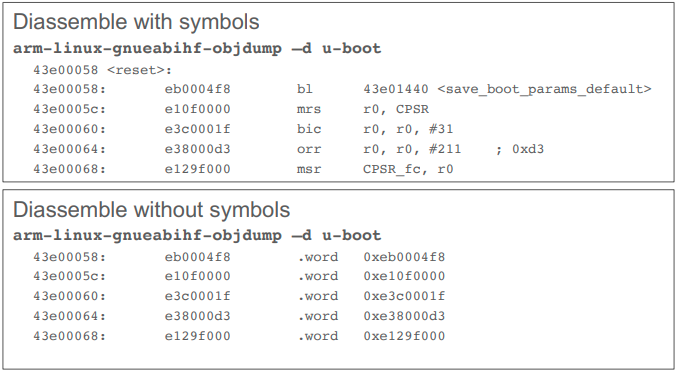
\includegraphics[width=0.9\columnwidth]{Figures/uboot_01.png}
\end{figure}

\subsection{Création de uImage}
uImage est l'image Linux au format uboot elle est créée lors du make. Dans le process du boot.cmd, uboot va spécifier son emplacement dans la variable d'environnement \verb!$kernel_addr_r=0x40080000!

\subsection{Flattened Device Tree}
Le FTD contient les informations sur le hardware que linux va utiliser pour sa configuration. Le fabricant du uP a surement écrit \verb!sun50i-h5-nanopi-neo-plus2.dts! et on le passe en \verb!.dtb! avec la commande \verb! dtc board.dts –o board.dtb!. Lors du boot.cmd on précise l'adresse de cd \verb!.dtb! dans la variable d'environnement \verb!$fdt_addr_r=0x4FA00000!

\subsection{Mapping de la SDCard}
La carte SD contient ces éléments
\begin{itemize}
\item \verb!sunxi-spl.bin!: Secondary Program Loader
\item \verb!u-boot.itb!: selon plus haut
\item \verb!boot!: image \verb!.ext4! qui contient 3 autres choses: \verb!Image!, \verb!nanopi-neo-plus2.dtb! et \verb!boot.scr!
\item \verb!rootfs!: le filesystem de linux
\end{itemize}

\subsection{boot.scr}
u-boot au démarrage, sans pression d'une touche, va chercher le fichier \verb!boot.scr! (format boot script) et l'exécuter. Il contient enfait les instructions du fichier \verb!boot.cmd!.
